\documentclass[../main.tex]{subfiles}
\begin{document}

\chapter{Lecture 10 - 07-04-2020}
\section{TO BE DEFINE}


\section{MANCANO 20 MINUTI DI LEZIONE}
$$ \barra{E}\left[z\right] = \barra{E}\left[ \, \barra{E} \left[ z\, |\, x \right]\, \right] \qquad \longrightarrow \quad \barra{E} \left[ Z \, | \, X= x \right] $$
\
$$\barra{E}\left[X\right] = \sum_{t = 1}^{m} \barra{E}\left[\, x \cdot \Pi\left(A\begin{small}
t \end{small} \right) \, \right] \qquad \bred{$A_1,..., A_m$ portion of sample law of total probability}$$
\\\
$$x \in \mathbb{R}^d \qquad
\mathbb{P}(Y_{\Pi(s,x)} = 1) = \\\\ \mathbb{E}\left[\Pi { Y_{\Pi(s,x)} = 1 } \right] = \qquad \bred{Law of total probability} 
$$
$$
= \sum_{t = 1}^{m} \, \mathbb{E}\left(\,\Pi\{Y_t = 1\} \, \cdot \, \Pi \cdot \, \{ \, \Pi(s,x) = t \} \, \right] \quad  =
$$
$$
= \quad \sum_{t = 1}^{m} \mathbb{E} \, \left[ \, \mathbb{E}\left[\,\Pi\{Y_t = 1\} \, \cdot \, \Pi \cdot \, \{\Pi(s,x) = t\}\, |\, X_t \, \right] \, \right] =
$$\\
given the fact that $Y_t \sim \eta(X_t) \Rightarrow$ give me probability \\
$$
Y_t = 1 \ \ and \ \ \Pi(s,x) = t \quad \textit{are independent given $X_Y$} \quad \left( \, e. g. \ \ \mathbb{E}\left[ Z\, X \right] = \mathbb{E}\left[x\right] \cdot \mathbb{E}\left[z \right] \  \right)
$$
$$
= \sum_{t = 1}^{m} \, \barra{E}\, \left[\barra{E} \, \left[ \,\Pi\{Y_t = 1\}\,|\,X_t \, \right] \cdot \barra{E} \left[ \, \Pi(s,x) = t | Xt \, \right] \, \right] \
= \ \sum_{t = 1}^{m} \barra{E}\left[\, \eta(X_t) \, \cdot \, \Pi \, \cdot \, \{\Pi (s,x) = t \} \, \right] = 
$$
$$
= \quad \barra{E} \left[ \, \eta \, (X_{\Pi(s,x)}\,)\right]
$$

$$ \barra{P} (Y_{\Pi(s,x)}| X=x = \barra{E}\left[\, \eta(X_\Pi (s,x)) \, \right] 
$$
\\

$$
\barra{P} (Y_{\Pi(s,x)} = 1, y = -1 ) = 
 \barra{E}\left[ \, \Pi\{Y_{\Pi(s,x)  }= 1\} \cdot \Pi \{Y= -1|X\} \, \right]\, ] =  \
$$
$$
= \barra{E}\left[ \, \Pi \{ Y_{\Pi(s,x)} = 1\} \cdot \Pi\{ y = -1 \} \, \right] 
= \barra{E}\left[ \, \barra{E}\left[ \,\Pi \{ Y_{\Pi(s,x)} = 1\} \cdot \Pi \{ y = -1 | X \} \, \right]\, \right] = 
$$
\bred{by independence i can split them }
$$
 Y_{\Pi(s,x)} = 1  \quad \quad y = -1 \bred{ \quad which is $ 1- \eta(x)$} \quad when \quad X = x 
$$

$$ = \barra{E}\left[ \, \barra{E}\left[ \, \Pi \{Y_\Pi(s,x)\} = 1 | X \, \right] \cdot \barra{E}\left[\, \Pi \{y = -1\} |X \, \right]\, \right] = \barra {E}\left[\, \eta_{\Pi(s,x)} \cdot (1-\eta(x))\, \right] =
$$

similarly:
$$
\barra{P}\left(Y_{\Pi(s,x)} = -1 ,  y = 1 \right) = \barra{E} \left[\, (1- \eta_{\Pi(s,x)}) \cdot \eta(x) \, \right]
$$\
$$
\barra{E} \left[\,  \ell_D (\hat{h}_s) \, \right] = \barra{P}\left(Y_{\Pi(s,x)} \neq y \right) = \barra{P}\left(Y_{\Pi(s,x)} = 1, y = -1\right) + \barra{P}\left(Y_{Pi(s,x)} = -1, y = 1\right) 
$$
$$
= \barra{E} \left[\, \eta_{\Pi(s,x)} \cdot (1-eta(x))\right] + \barra{E}\left[\,( 1- \eta_{\Pi(s,x)})\cdot \eta(x)\, \right]
$$
\\
\bred{
Make assumptions on $D_x \quad and \quad \eta$: }\\
\begin{enumerate}
\item $\forall X$ drawn from $D_x$ \quad $\max |X_t| \leq 1$\\
Feature values are bounded in $[-1,1]$\\
all my points belong to this:$$
X = \left[-1,1\right]^d
$$
\item $\eta$ is such that $\exists c < \infty$ :\\
$$
\eta(x) - \eta(x') \, \leq \, c \cdot \| X-x' \| \quad \forall \, x,x' \in X
$$
It means that $\eta$ is \bred{Lipschitz} in $X$ 
$c <\infty \Leftrightarrow$ $\eta$ is continous\\
\end{enumerate}
\bred{using two facts:}\\
\begin{figure}[h]
    \centering
    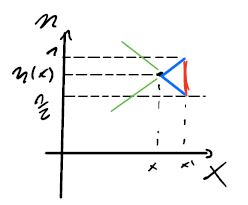
\includegraphics[width=0.6\linewidth]{../img/lez10-img1.JPG}
    \caption{Point (2) - where \quad $y = cx +q$ \qquad  $y = -cx +q $}
\end{figure}
$$
\eta(x') \leq \eta(x) + c \, || X-x'|| \quad \longrightarrow \quad  \bred{euclidean distance}
$$
$$
1-\eta(x') \leq 1- \eta(x) + c \, ||X-x'||
\\\\
$$\
$
X' = X_{\Pi(s,x)}
$
$$
\eta(X) \cdot \left(1-\eta(x')\right) + \left(1-\eta(x)\right)\cdot \eta(x') \leq
$$
$$
\leq \eta(x) \cdot((1-\eta(x))+\eta(x)\cdot c \, ||X-x'|| + (1-\eta(x))\cdot c \, ||X-x'|| = 
$$
$$
= 2 \cdot \eta(x) \cdot (1- \eta(x)) + c\, ||X-x'|| 
$$\
$$
\barra{E}\left[\ell_d \cdot (\hat{h}_s)\right] \leq 
2 \cdot \barra{E} \left[\, \eta(x) - (1-\eta(x))\, \right] + c \cdot \barra(E)\left[\, ||X-x_{\Pi(s,x)}||\, \right]
$$
where $\leq$ mean at most
\\\\
\section{Compare risk for zero-one loss}
$$
\barra{E}\left[\, \min\{\eta(x),1-\eta(x)\} \, \right] = \ell_D (f^*) $$
$$
\eta(x) \cdot( 1- \eta(X)) \ \leq \ \min\{ \,\eta(x), 1-\eta(x)\, \} \quad \forall x
$$
$$
\barra{E}\left[\, \eta(x)\cdot(1-\eta(x)\, \right] \ \leq  \ \ell_D(f^*)
$$
$$
\barra{E}\left[\, \ell_d(\hat{l}_s)\, \right] \leq 2 \cdot \ell_D(f^*) + c \cdot \barra{E}\left[\, \|X-X_{\Pi(s,x)}\| \, \right]
\\\\
\eta(x) \in \{0,1\}
$$
\\
Depends on dimension: \bred{curse of dimensionality}
\\
\begin{figure}[h]
    \centering
    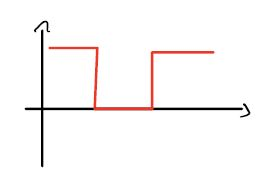
\includegraphics[width=0.6\linewidth]{../img/lez10-img2.JPG}
    \caption{Point}
\end{figure}\\
$
\ell_d(f^*) = 0 \iff \min\{ \eta(x), 1-\eta(x)\} =0 \quad$ with probability = 1
\\
to be true $\eta(x) \in \{0,1\}$

\end{document}